A Figura~\ref{fig:hiper} apresenta a mediana de 51 rodadas de resposta do algoritmo xNES a variações tanto do
tamanho da população, quanto da taxa de aprendizado $\eta_A$.
Diferentemente da matriz $A$ que pertence ao $\mathbb{R}^{d \times d}$, o valor $\mu$ pertence ao $\mathbb{R}^{d}$, sendo
mais fácil de ser encontrado adaptativamente.
Portanto, o parâmetro $\eta_{\mu}$ não foi mantido com valor recomendado.

A partir da Figura~\ref{fig:hiper}, pode-se fazer algumas considerações.
Percebe-se que para baixos valores de $\eta_A$, como $0,0033$, o algoritmo tem seu pior desempenho em todas as funções
de avaliação, com exceção da Função 14.
Esse pode ser um indicativo que para este valor de taxa de aprendizado o algoritmo necessite de mais avaliações para
obter sucesso.

Para populações com maior número de indivíduos, maiores taxas de aprendizado costumam ser melhores mas novamente a Função 14
não apresenta esse comportamento.
Uma possível explicação para esse fenômeno é encontrada na maior pressão nos indivíduos devido ao tamanho da população, sendo
assim o algoritmo beneficiado pela maior capacidade exploratória provinda de altas taxas de aprendizado.

Outra observação a ser feita em relação ao tamanho da população: utilizando-se menos indivíduos, $8$ ou $13$, taxas de
aprendizado baixas ou altas demais resultam em pior performance quando comparadas a utilização de valores como $0,02$ ou
$0.033$.

Conclui-se que, dada a variedade de funções objetivo e as diferentes dimensionalidades, não se pode apontar um vencedor absoluto.
Funções distintas se sobressaem com diferentes parâmetros.
Entretanto, notou-se que a combinação de parâmetros que melhor generalizou foi a de tamanho $21$ de população e taxa de
aprendizado $\eta_A = 0,033$.
Sendo assim, o tamanho de população consideravelmente maior que o proposto originalmente.
Uma possível explicação para as vantagens obtidas com essa configuração é que devido ao maior número de indivíduos se obtém
melhore estimações do gradiente natural do erro.

\begin{figure*}[!t]
\centering
\subfloat{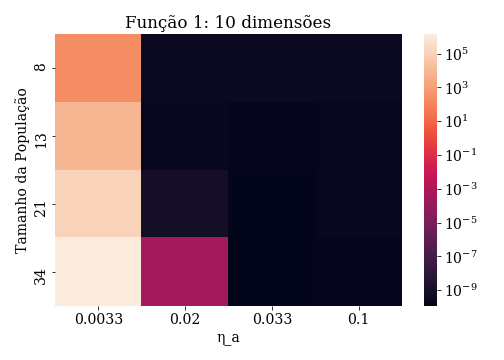
\includegraphics[width=2.0in]{figures/hiper_selection/function=01_dim=10.png}
\label{fig:func01dim10}}
\subfloat{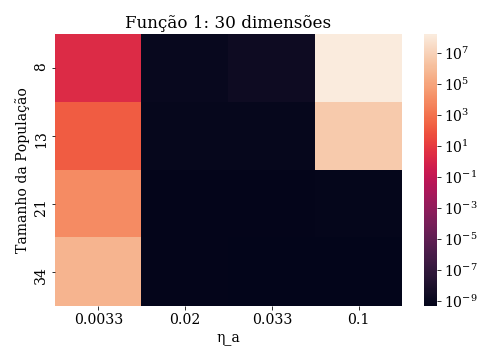
\includegraphics[width=2.0in]{figures/hiper_selection/function=01_dim=30.png}
\label{fig:func01dim30}}
\hfil
\subfloat{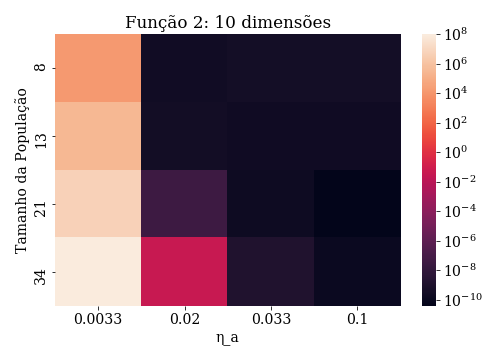
\includegraphics[width=2.0in]{figures/hiper_selection/function=02_dim=10.png}
\label{fig:func02dim10}}
\subfloat{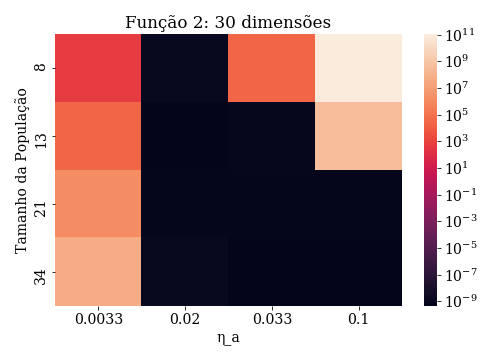
\includegraphics[width=2.0in]{figures/hiper_selection/function=02_dim=30.png}
\label{fig:func02dim30}}
\hfil
\subfloat{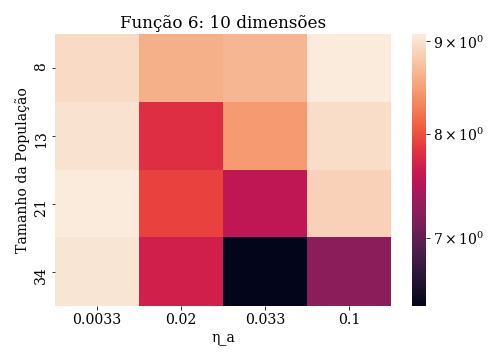
\includegraphics[width=2.0in]{figures/hiper_selection/function=06_dim=10.png}
\label{fig:func06dim10}}
\subfloat{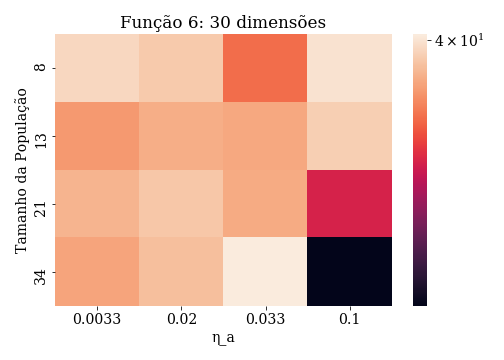
\includegraphics[width=2.0in]{figures/hiper_selection/function=06_dim=30.png}
\label{fig:func06dim30}}
\hfil
\subfloat{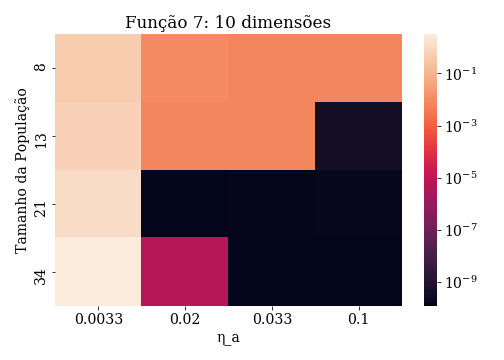
\includegraphics[width=2.0in]{figures/hiper_selection/function=07_dim=10.png}
\label{fig:func07dim10}}
\subfloat{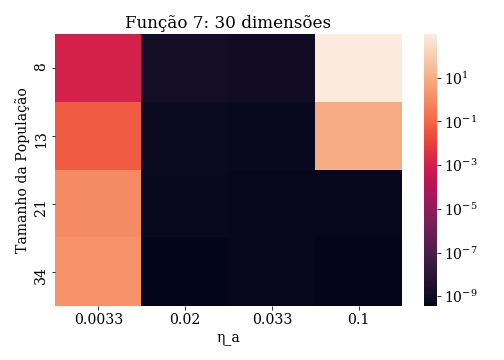
\includegraphics[width=2.0in]{figures/hiper_selection/function=07_dim=30.png}
\label{fig:func07dim30}}
\hfil
\subfloat{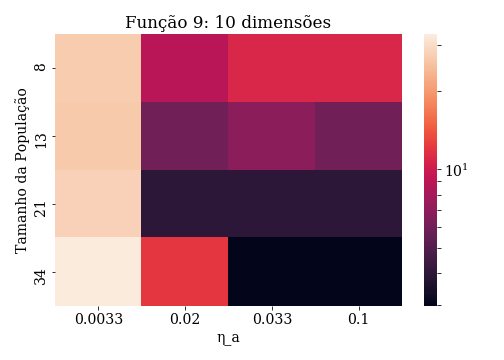
\includegraphics[width=2.0in]{figures/hiper_selection/function=09_dim=10.png}
\label{fig:func09dim10}}
\subfloat{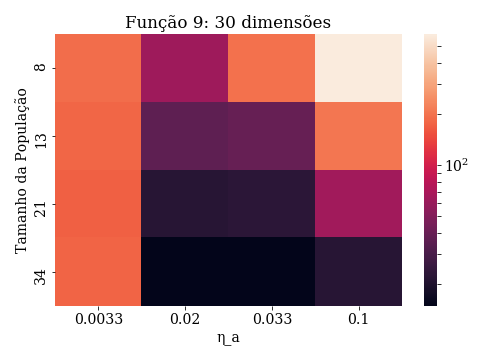
\includegraphics[width=2.0in]{figures/hiper_selection/function=09_dim=30.png}
\label{fig:func09dim30}}
\hfil
\subfloat{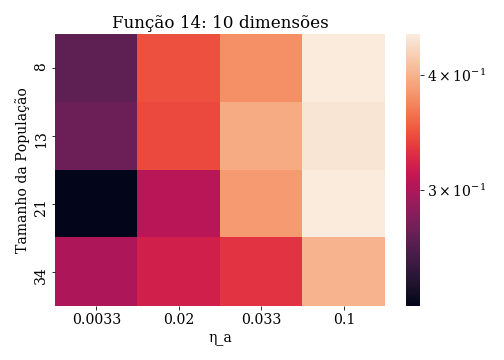
\includegraphics[width=2.0in]{figures/hiper_selection/function=14_dim=10.png}
\label{fig:func14dim10}}
\subfloat{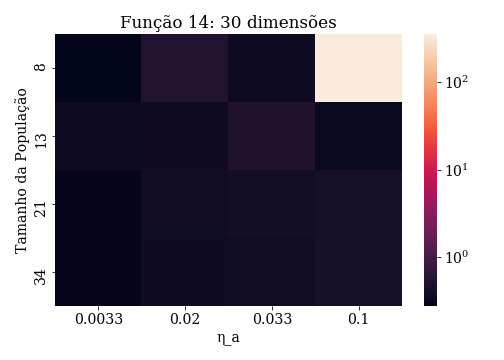
\includegraphics[width=2.0in]{figures/hiper_selection/function=14_dim=30.png}
\label{fig:func14dim30}}
\caption{Seleção de hiperparâmetros do xNES}
\label{fig:hiper}
\end{figure*}

Seguindo para a fase de comparação entre os algoritmos, a Figura~\ref{fig:comp} apresenta o erro de aptidão obtido por
cada algoritmo.
Nessa figura comparamos o xNES com os parâmetros selecionados na fase anterior, o xNES com valores originalmente
apresentados pelos autores e o CMA-ES também com seus valores padrão.
Assim como na etapa anterior, cada algoritmo foi rodado 51 vezes para cada função.
Os resultados também estão dispostos nas Tabelas~\ref{tab:results_xnes_10}, \ref{tab:results_xnes_30},
\ref{tab:results_xnes_orig_10}, \ref{tab:results_xnes_orig_10}, \ref{tab:results_cmaes_10} e \ref{tab:results_cmaes_30}.

A primeira consideração a se feita é que para as funções $1$ e $2$ todos algoritmos foram capazes de obter sucesso, ou seja,
erro menor que $10^{-8}$, dentro do número permitido de avaliações da função objetivo.
Observamos ainda nas funções $1$ e $2$ que o algoritmo xNES com parâmetros pré-selecionados apresentou menor média e
variância de aptidão.

Analisando a função $6$, ressalta-se que o algoritmo CMA-ES foi o único a conseguir obter sucesso no problema com $10$
dimensões, porém em apenas uma das 51 rodadas.
Considerando ainda as $10$ dimensões, o CMA-ES superou o xNES com valores originais, porém, esta dentro da margem de
erro do xNES com parâmetros selecionados, apesar de apresentar menor média de erro.
Por sua vez, para função $7$ com $30$ dimensões o CMA-ES superou os outros dois algoritmos que apresentaram resultados
iguais entre si.

A função $7$ apresenta um comportamento atípico, os resultados obtidos em $30$ dimensões para todos algoritmos foram superiores
aos resultados de $10$ dimensões.
Nesta função a variação de parâmetros do xNES se mostrou irrelevante.
Analisando o problema com 10 dimensões, o CMA-ES apresentou a maior média de erro e obteve sucesso apenas em 25\% das
rodadas enquanto os xNES obtiveram 50\% de sucesso, porém, os resultados ainda se encontram dentro da barra de erro.
Avaliando o problema com $30$ dimensões os xNES obtiveram sucesso em todos os casos enquanto o CMA-ES atingiu o 84\% das rodadas.

As funções $9$ e $14$ apresentam resultados parecidos entre todos algoritmos.
Nestas avaliações todos algoritmos apresentaram resultados dentro das margens de erro.

Os experimentos foram executados em um computador com 8 CPUs e totalizaram 50 minutos de processamento.

\begin{figure*}[!t]
\centering
\subfloat{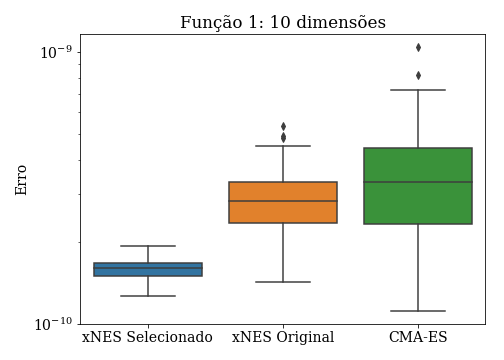
\includegraphics[width=2.0in]{figures/analysis_results/function=01_dim=10.png}
\label{fig:result_func01dim10}}
\subfloat{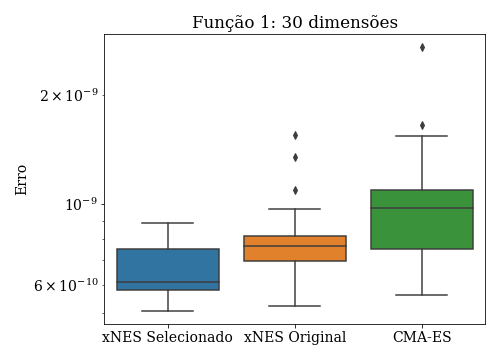
\includegraphics[width=2.0in]{figures/analysis_results/function=01_dim=30.png}
\label{fig:result_func01dim30}}
\hfil
\subfloat{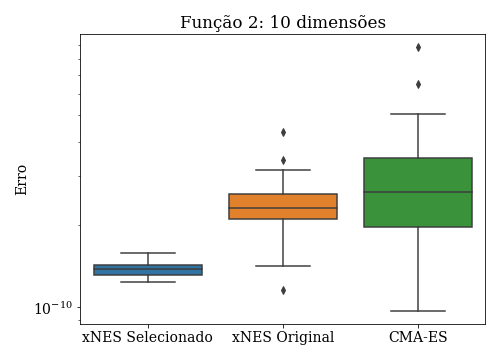
\includegraphics[width=2.0in]{figures/analysis_results/function=02_dim=10.png}
\label{fig:result_func02dim10}}
\subfloat{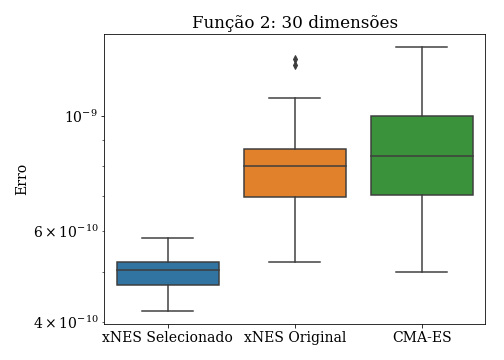
\includegraphics[width=2.0in]{figures/analysis_results/function=02_dim=30.png}
\label{fig:result_func02dim30}}
\hfil
\subfloat{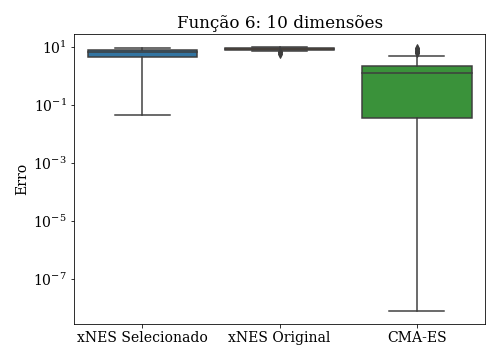
\includegraphics[width=2.0in]{figures/analysis_results/function=06_dim=10.png}
\label{fig:result_func06dim10}}
\subfloat{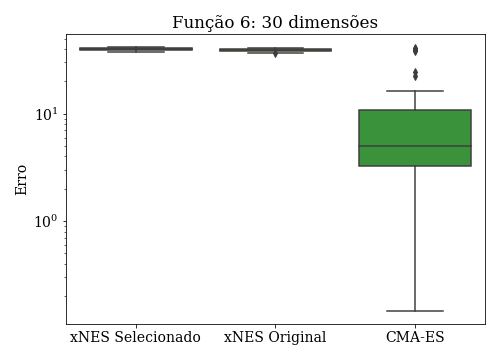
\includegraphics[width=2.0in]{figures/analysis_results/function=06_dim=30.png}
\label{fig:result_func06dim30}}
\hfil
\subfloat{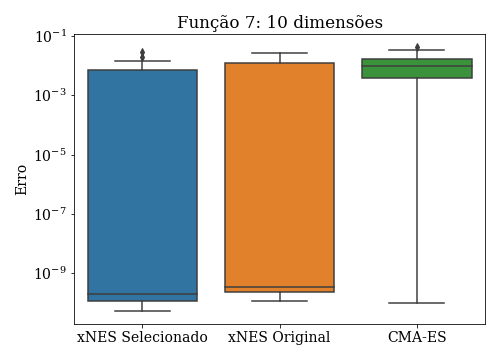
\includegraphics[width=2.0in]{figures/analysis_results/function=07_dim=10.png}
\label{fig:result_func07dim10}}
\subfloat{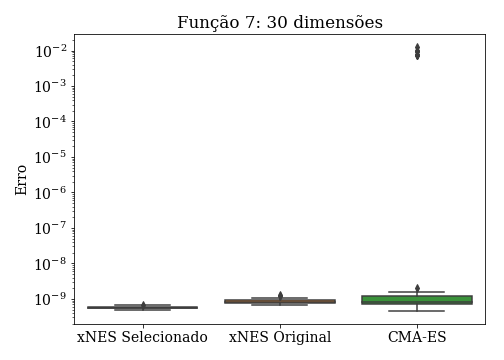
\includegraphics[width=2.0in]{figures/analysis_results/function=07_dim=30.png}
\label{fig:result_func07dim30}}
\hfil
\subfloat{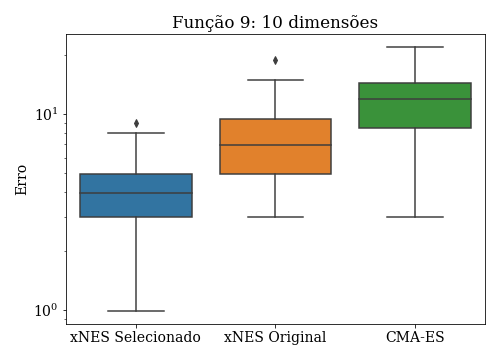
\includegraphics[width=2.0in]{figures/analysis_results/function=09_dim=10.png}
\label{fig:result_func09dim10}}
\subfloat{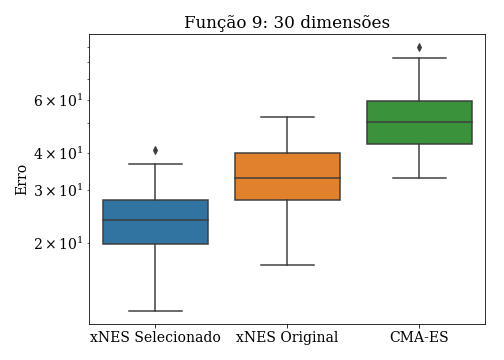
\includegraphics[width=2.0in]{figures/analysis_results/function=09_dim=30.png}
\label{fig:result_func09dim30}}
\hfil
\subfloat{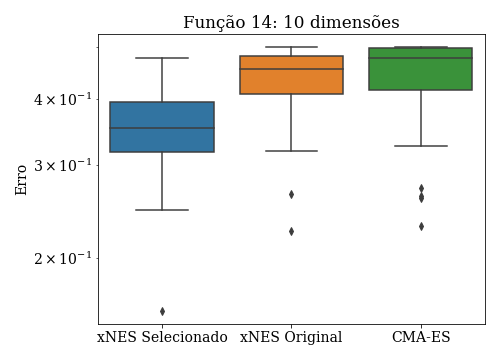
\includegraphics[width=2.0in]{figures/analysis_results/function=14_dim=10.png}
\label{fig:result_func14dim10}}
\subfloat{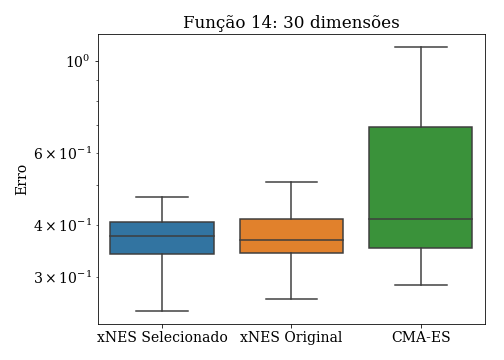
\includegraphics[width=2.0in]{figures/analysis_results/function=14_dim=30.png}
\label{fig:result_func14dim30}}
\caption{Comparação entre os algoritmos}
\label{fig:comp}
\end{figure*}


\begin{table}[!t]
\renewcommand{\arraystretch}{1.3}
\caption{xNES Selecionado - 10 Dimensões}
\label{tab:results_xnes_10}
\centering
\resizebox{\columnwidth}{!}{%
\begin{tabular}{|l|r|r|r|r|r|r|}
\hline
Função &    Melhor   &      Pior &   Mediana &     Média &  \specialcell{Desvio\\Padrão} &  \specialcell{Taxa de\\ Sucesso} \\
\hline
1        &  1.27e-10 &  1.93e-10 &  1.60e-10 &  1.60e-10 &      1.32e-11 &             1.00 \\
2        &  1.23e-10 &  1.58e-10 &  1.38e-10 &  1.38e-10 &      8.72e-12 &             1.00 \\
6        &  4.51e-02 &  9.39e+00 &  6.73e+00 &  6.09e+00 &      2.48e+00 &             0.00 \\
7        &  5.30e-11 &  2.96e-02 &  2.01e-10 &  4.98e-03 &      6.21e-03 &             0.51 \\
9        &  9.95e-01 &  8.95e+00 &  3.98e+00 &  4.14e+00 &      1.81e+00 &             0.00 \\
14       &  1.59e-01 &  4.77e-01 &  3.52e-01 &  3.49e-01 &      6.10e-02 &             0.00 \\
\hline
\end{tabular}
}
\end{table}

\begin{table}[!t]
\renewcommand{\arraystretch}{1.3}
\caption{xNES Selecionado - 30 Dimensões}
\label{tab:results_xnes_30}
\centering
\resizebox{\columnwidth}{!}{%
\begin{tabular}{|l|r|r|r|r|r|r|}
\hline
Função &    Melhor   &      Pior &   Mediana &     Média &  \specialcell{Desvio\\Padrão} &  \specialcell{Taxa de\\ Sucesso} \\
\hline
1        &  5.09e-10 &  8.84e-10 &  6.12e-10 &  6.60e-10 &       1.04e-10 &              1.00 \\
2        &  4.21e-10 &  5.82e-10 &  5.04e-10 &  4.98e-10 &       3.68e-11 &              1.00 \\
6        &  3.75e+01 &  4.16e+01 &  3.97e+01 &  3.97e+01 &       1.05e+00 &              0.00 \\
7        &  4.86e-10 &  6.92e-10 &  5.65e-10 &  5.75e-10 &       4.89e-11 &              1.00 \\
9        &  1.19e+01 &  4.08e+01 &  2.39e+01 &  2.44e+01 &       6.47e+00 &              0.00 \\
14       &  2.48e-01 &  4.69e-01 &  3.77e-01 &  3.72e-01 &       4.94e-02 &              0.00 \\
\hline
\end{tabular}
}
\end{table}

\begin{table}[!t]
\renewcommand{\arraystretch}{1.3}
\caption{xNES Original - 10 Dimensões}
\label{tab:results_xnes_orig_10}
\centering
\resizebox{\columnwidth}{!}{%
\begin{tabular}{|l|r|r|r|r|r|r|}
\hline
Função &    Melhor   &      Pior &   Mediana &     Média &  \specialcell{Desvio\\Padrão} &  \specialcell{Taxa de\\ Sucesso} \\
\hline
1        &  1.42e-10 &  5.34e-10 &  2.82e-10 &  2.98e-10 &      8.84e-11 &             1.00 \\
2        &  1.16e-10 &  4.34e-10 &  2.30e-10 &  2.37e-10 &      5.39e-11 &             1.00 \\
6        &  5.95e+00 &  9.91e+00 &  8.79e+00 &  8.59e+00 &      8.29e-01 &             0.00 \\
7        &  1.14e-10 &  2.71e-02 &  3.46e-10 &  6.13e-03 &      7.42e-03 &             0.51 \\
9        &  2.98e+00 &  1.89e+01 &  6.96e+00 &  7.53e+00 &      3.45e+00 &             0.00 \\
14       &  2.24e-01 &  5.00e-01 &  4.55e-01 &  4.38e-01 &      6.00e-02 &             0.00 \\
\hline
\end{tabular}
}
\end{table}

\begin{table}[!t]
\renewcommand{\arraystretch}{1.3}
\caption{xNES Original - 30 Dimensões}
\label{tab:results_xnes_orig_30}
\centering
\resizebox{\columnwidth}{!}{%
\begin{tabular}{|l|r|r|r|r|r|r|}
\hline
Função &    Melhor   &      Pior &   Mediana &     Média &  \specialcell{Desvio\\Padrão} &  \specialcell{Taxa de\\ Sucesso} \\
\hline
1        &  5.23e-10 &  1.54e-09 &  7.66e-10 &  7.83e-10 &       1.73e-10 &              1.00 \\
2        &  5.22e-10 &  1.29e-09 &  7.99e-10 &  7.98e-10 &       1.50e-10 &              1.00 \\
6        &  3.65e+01 &  4.12e+01 &  3.96e+01 &  3.94e+01 &       1.08e+00 &              0.00 \\
7        &  6.62e-10 &  1.28e-09 &  8.43e-10 &  8.52e-10 &       1.27e-10 &              1.00 \\
9        &  1.69e+01 &  5.27e+01 &  3.28e+01 &  3.43e+01 &       8.65e+00 &              0.00 \\
14       &  2.64e-01 &  5.09e-01 &  3.68e-01 &  3.87e-01 &       7.12e-02 &              0.00 \\
\hline
\end{tabular}
}
\end{table}

\begin{table}[!t]
\renewcommand{\arraystretch}{1.3}
\caption{CMA-ES - 10 Dimensões}
\label{tab:results_cmaes_10}
\centering
\resizebox{\columnwidth}{!}{%
\begin{tabular}{|l|r|r|r|r|r|r|}
\hline
Função &    Melhor   &      Pior &   Mediana &     Média &  \specialcell{Desvio\\Padrão} &  \specialcell{Taxa de\\ Sucesso} \\
\hline
1        &  1.12e-10 &  1.04e-09 &  3.31e-10 &  3.57e-10 &       1.80e-10 &             1.00 \\
2        &  9.73e-11 &  8.84e-10 &  2.64e-10 &  2.88e-10 &       1.39e-10 &             1.00 \\
6        &  7.88e-09 &  9.13e+00 &  1.24e+00 &  2.06e+00 &       2.49e+00 &             0.02 \\
7        &  9.66e-11 &  4.18e-02 &  9.86e-03 &  1.16e-02 &       1.03e-02 &             0.25 \\
9        &  2.98e+00 &  2.19e+01 &  1.19e+01 &  1.16e+01 &       4.64e+00 &             0.00 \\
14       &  2.30e-01 &  5.00e-01 &  4.77e-01 &  4.44e-01 &       7.38e-02 &             0.00 \\
\hline
\end{tabular}
}
\end{table}

\begin{table}[!t]
\renewcommand{\arraystretch}{1.3}
\caption{CMA-ES - 30 Dimensões}
\label{tab:results_cmaes_30}
\centering
\resizebox{\columnwidth}{!}{%
\begin{tabular}{|l|r|r|r|r|r|r|}
\hline
Função &    Melhor   &      Pior &   Mediana &     Média &  \specialcell{Desvio\\Padrão} &  \specialcell{Taxa de\\ Sucesso} \\
\hline
1        &  5.60e-10 &  2.70e-09 &  9.74e-10 &  9.84e-10 &       3.43e-10 &             1.00 \\
2        &  5.00e-10 &  1.36e-09 &  8.35e-10 &  8.63e-10 &       2.06e-10 &             1.00 \\
6        &  1.47e-01 &  4.10e+01 &  5.04e+00 &  9.99e+00 &       1.20e+01 &             0.00 \\
7        &  4.65e-10 &  1.23e-02 &  8.22e-10 &  1.40e-03 &       3.35e-03 &             0.84 \\
9        &  3.28e+01 &  8.95e+01 &  5.07e+01 &  5.27e+01 &       1.31e+01 &             0.00 \\
14       &  2.87e-01 &  1.08e+00 &  4.15e-01 &  5.14e-01 &       2.00e-01 &             0.00 \\
\hline
\end{tabular}
}
\end{table}
